\section{Оборудование}
\begin{figure}[ht!]
    \center{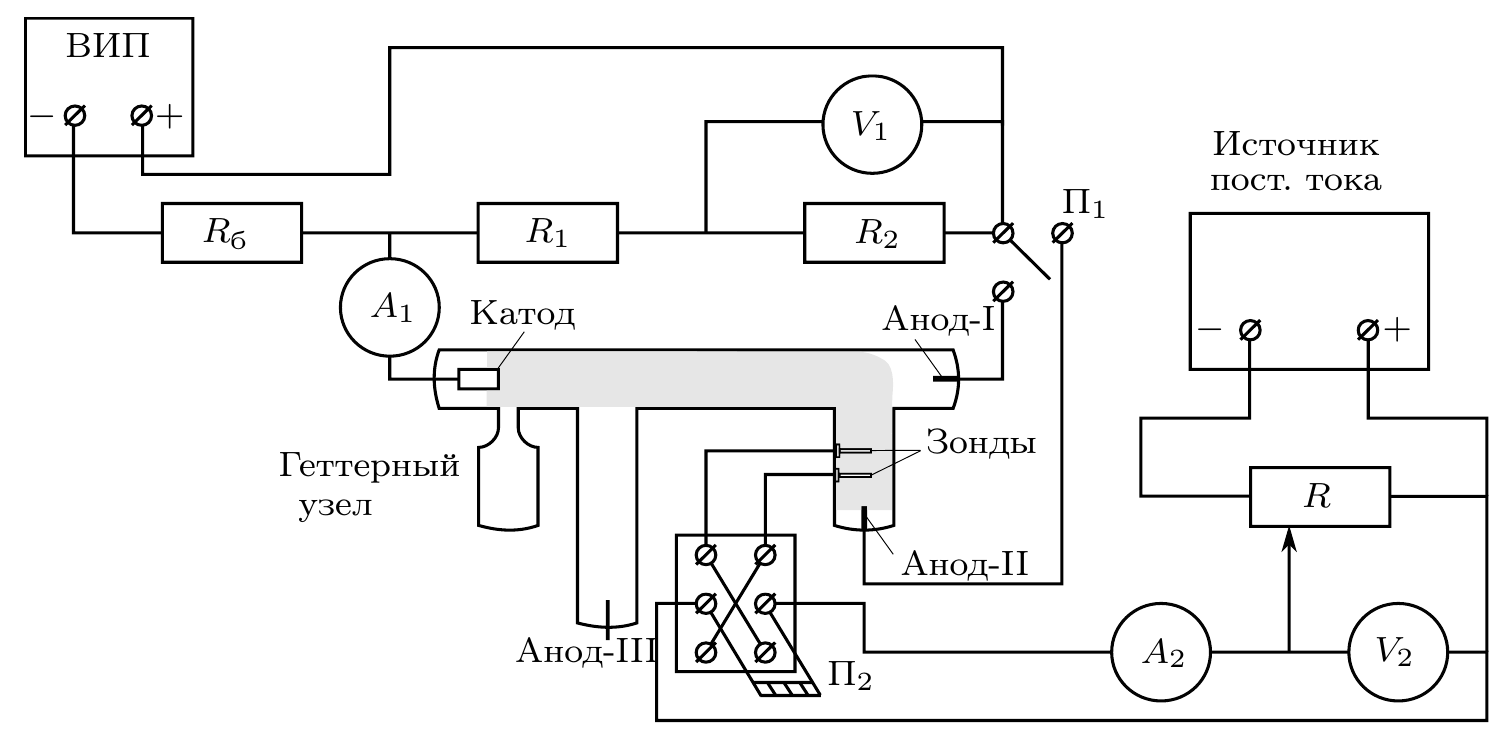
\includegraphics[width=0.8\linewidth]{../img/eq1.png}}
\end{figure}

Схема установки приведена на рисунке. Стеклянная газоразрядная трубка имеет холодный полый катод, три анода и геттерный узел~--- 
стеклянный баллон, на внутреннюю поверхность которого напылена газопоглощающая плёнка (геттер). Трубка наполнена изотопом неона
$^{22}\text{Ne}$ при давлении 2 мм рт.ст. Катод и один из анодов с помощью выключателя $\text{П}_{1}$  подключаются через балластный резистор
$R_{\text{б}}\approx 500\,\text{КОм}$ к регулируемому высоковольтному источнику питания (ВИП) с выходным напряжением до нескольких киловольт.

При подключении к ВИП анода-\rom{1} между  ним и катодом возникает газовый разряд. Ток разряда измеряется миллиамперметром $A_{1}$,
а падение напряжения на разрядной трубке~--- вольтметром $V_{1}$, подключённым к трубке через высоковольтный (несколько МОм) делитель
напряжения с коэффициентом $\left(R_{1} + R_{2}\right)/R_{2}$.

При подключении к ВИП анода-\rom{2} разряд возникает в пространстве между катодом и анодом-\rom{2}, где  находится двойной зонд, используемый
для диагностики плазмы положительного столба. Зонды изготовлены из молибденовой проволоки диаметром $d$ и имеют длину $l$.
Они подключены к источнику питания через потенциометр $R$. Переключатель $\text{П}_{2}$ позволяет изменять полярность напряжения на зондах.
Величина напряжения на зондах изменяется с помощью дискретного переключателя <<$V$>> выходного напряжения источника питания и потенциометра $R$,
а измеряется вольтметром $V_{2}$. Для измерения зондового тока используется микроамперметр $A_{2}$. Анод-\rom{3} в работе не используется.

